\section{Results}
%
\colorbox{yellow}{Need something about how this was run on Kongull?}\\
First it is important to verify that the code works correctly. This was done by comparing the results to an analytical solution and plotting the error for different problem sizes $n$. The problem chosen for this task was 
\begin{align}
  \label{eq:conv} 
  f = 5 \pi^2 \sin (\pi x) \sin (2 \pi y),
\end{align}
with the solution
\begin{align}
  u = \sin (\pi x) \sin (2 \pi y). 
\end{align}
The max norm was used to measure the error. The calculations were run with two threads on 1, 3 and 6 MPI processes, and the results can be found in Figure~\ref{fig:errVsn}. This plot is a log-log plot, with a reference line of slope $-2$. As the points follow the line, this means the method has quadratic converges. As the numerical scheme is a second order method, the figure confirms that our implementation is correct. For the rest of this section all tests are done with the $f$ in Eq.~\eqref{eq:conv}, unless specified otherwise.\\
%
\begin{figure}[h!]
\begin{center}
    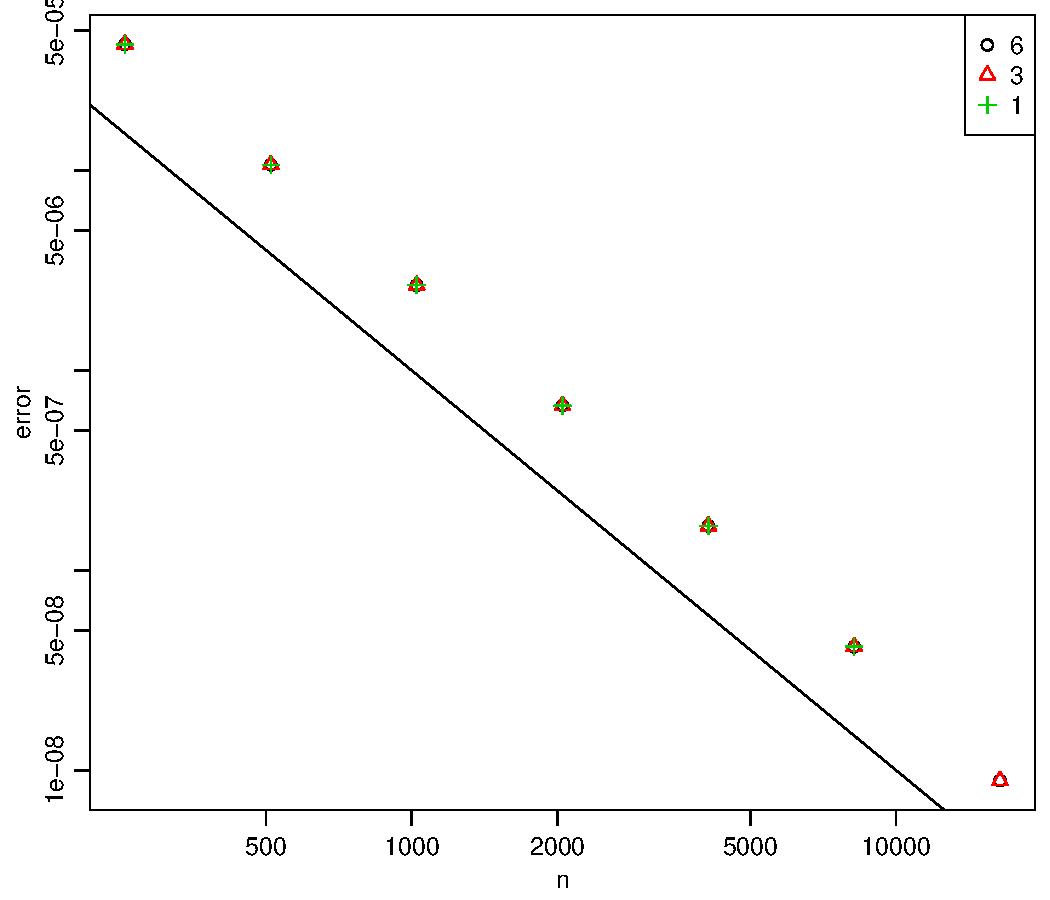
\includegraphics[scale=0.4]{./Figures/errVsn.pdf}
\end{center}
  \vspace{-1\baselineskip}
\caption{Loglog plot of the error as function of $n$. A reference line with slpe $-2$ is drawn. The problem in run on two threads with the number of processes specified in the legend.}
\label{fig:errVsn}
\end{figure}
%
\\
Next the problem was run on a single node where all 12 processors were utilized. The point was to investigate the performance of using threads versus MPI processes. Thus the relation between threads $t$ and processes $p$ is $p t = 12$ or $p = 12/t$. The calculations were done with $n = 2^{14} = 16384$. 
The same problem was repeated on three nodes where all 12 processors were utilized in the same way as above. The results can be found in Figure~\ref{fig:taskc}. Immediately it is clear there the times are pretty noisy. This is important to take into account later in the report, where the problem is only run once for each test case. It is clear from both plots that it is preferable to use only MPI processes and no openMP. 

While running only one MPI process and 12 threads on one node there is still some overhead from the MPI sending to itself and the work of reordering the data. Therefore the problem was solved on 12 threads without this overhead. The results are the red crosses in Figure~\ref{fig:taskc}. It is clear that it is a lot faster than with the MPI sending, but it is still slower than running with 12 MPI processes. 
\\
\begin{figure}[h!]
  \centering
  \begin{subfigure}[b]{0.48\textwidth}
    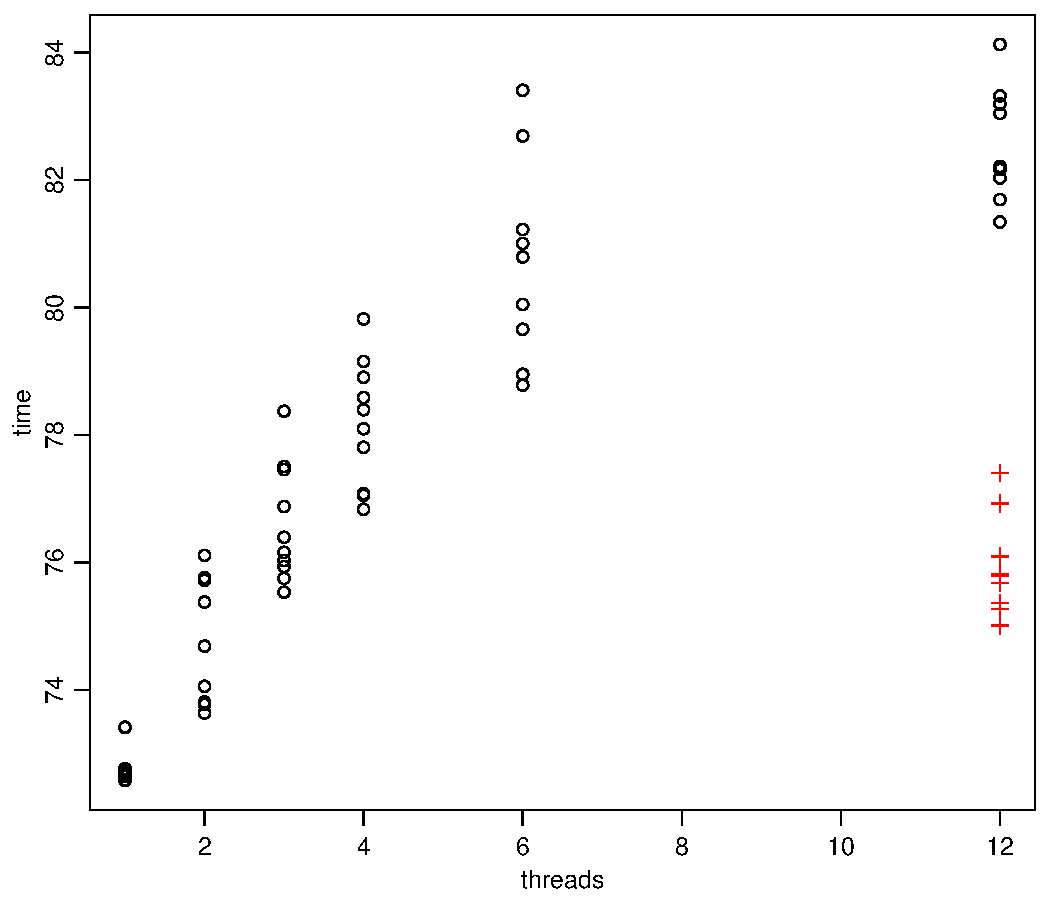
\includegraphics[width=\textwidth]{./Figures/taskc1.pdf}
  \end{subfigure}%
  \quad
  \begin{subfigure}[b]{0.48\textwidth}
    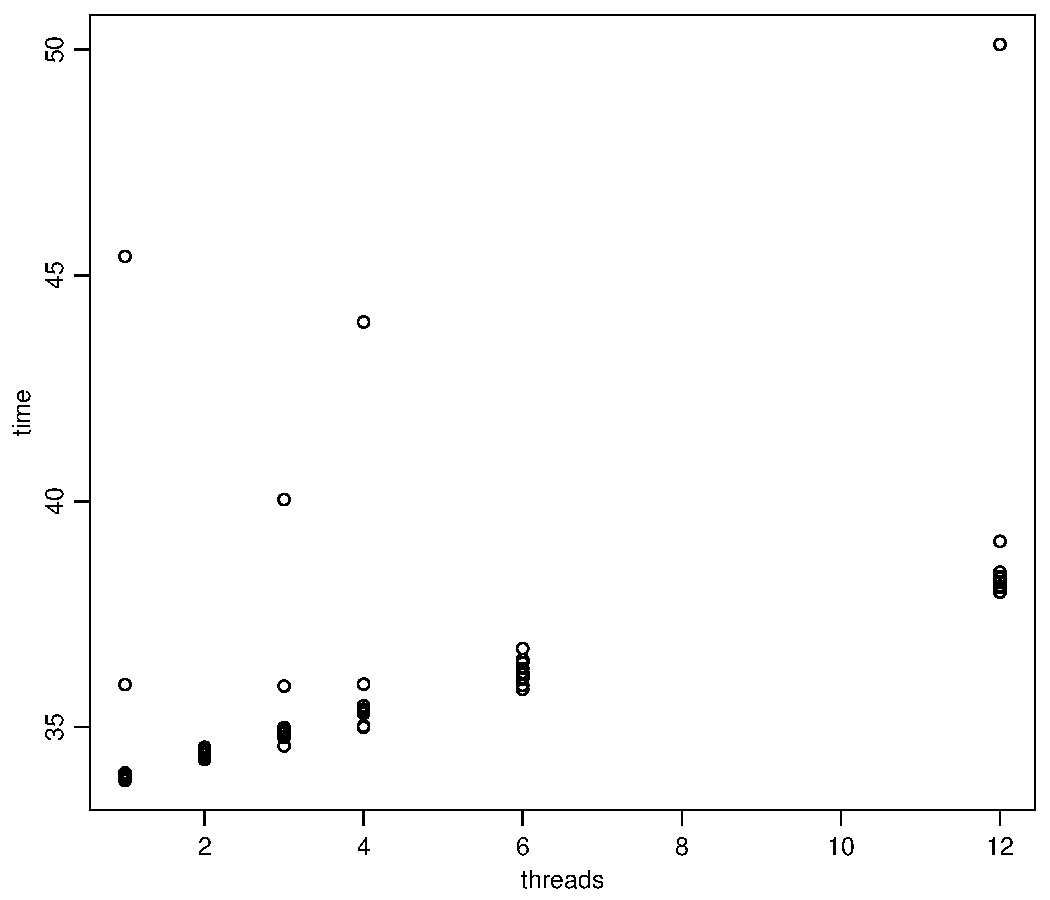
\includegraphics[width=\textwidth]{./Figures/taskc2.pdf}
  \end{subfigure}
          %(or a blank line to force the subfigure onto a new line)
  \vspace{-0.1\baselineskip}
  \caption{Times (in seconds) for running MPI processes vs threads with $n = 2^{14}$. The total number of processors used are 12 per node, so the number of processes per node is 12 - threads. The left figure is run on one node, while the right is run on three nodes. The red crosses are run without any MPI sending at all.}
  \label{fig:taskc}
\end{figure}
\\
Next timing results were obtained by running the problem on different number of processes with one thread. Here up to three nodes were used, and a new node was only used if when there were no more free processors in the previous nodes. This was done for different problem sizes and plotted in Figure~\ref{fig:time1}. Sending between processes on a node should be faster than sending between nodes. This trend is clear in the figure, as the first points after utilizing an extra node (after the vertical lines), clearly do not follow the trend of the previous points. In Figure~\ref{fig:time2}, the same experiment is done, but with two treads instead of one. So here only up to 6 MPI processes were used on each node. Although it is clear from Figure~\ref{fig:taskc} that this should be worse than only using MPI processes, it is hard to distinguish Figure~\ref{fig:time1} and Figure~\ref{fig:time2}. To investigate how the time changed with only using threads on each node, the problem was run on 1 to 12 threads on 1 to three nodes. In Figure~\ref{fig:time3} this is plotted and we see the behavior is the same as in the other figures. It is reasonable to assume that for if run on more nodes, the time would eventually start to grow because of the overhead. There are some larger times at the end of Figure~\ref{fig:time1}, but this is probably just noise.\\
%
\begin{figure}[h!]
  \centering
  \begin{subfigure}[b]{0.48\textwidth}
    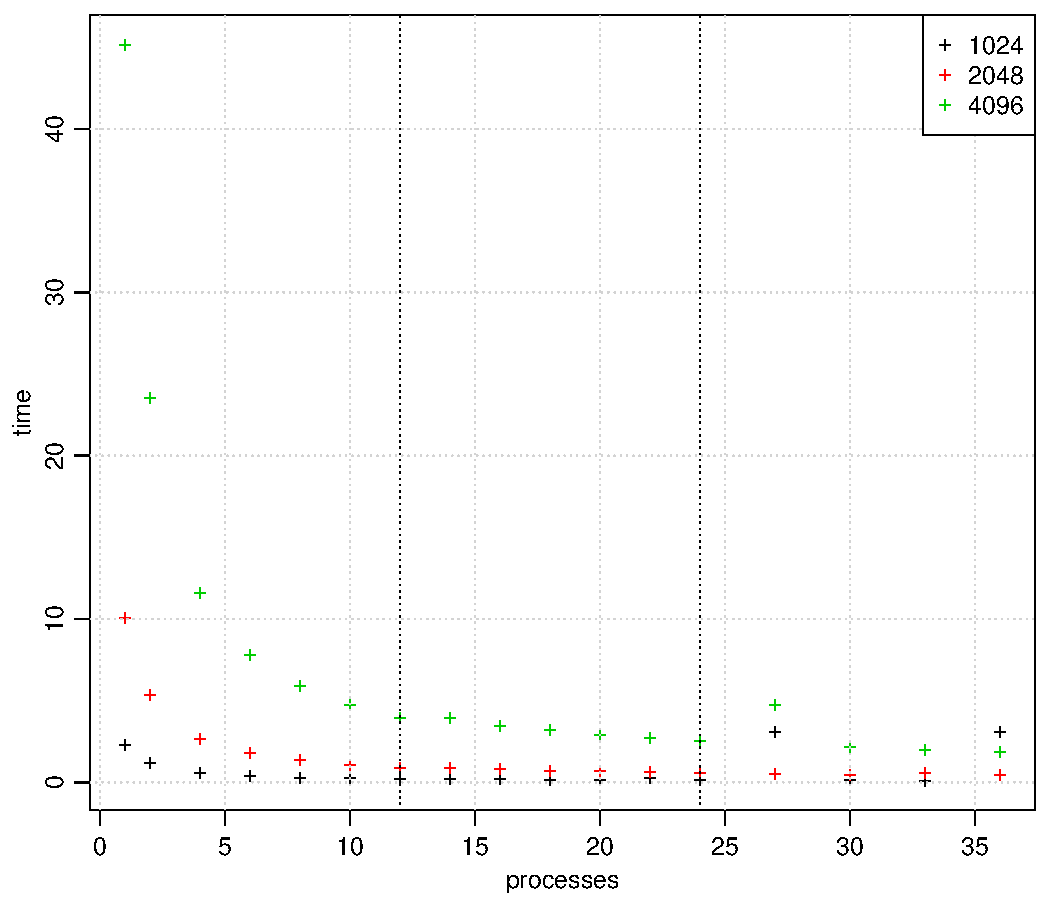
\includegraphics[width=\textwidth]{./Figures/taskbTimeProc1.pdf}
    \caption{}
    \label{fig:time1}
  \end{subfigure}%
  \quad
  \begin{subfigure}[b]{0.48\textwidth}
    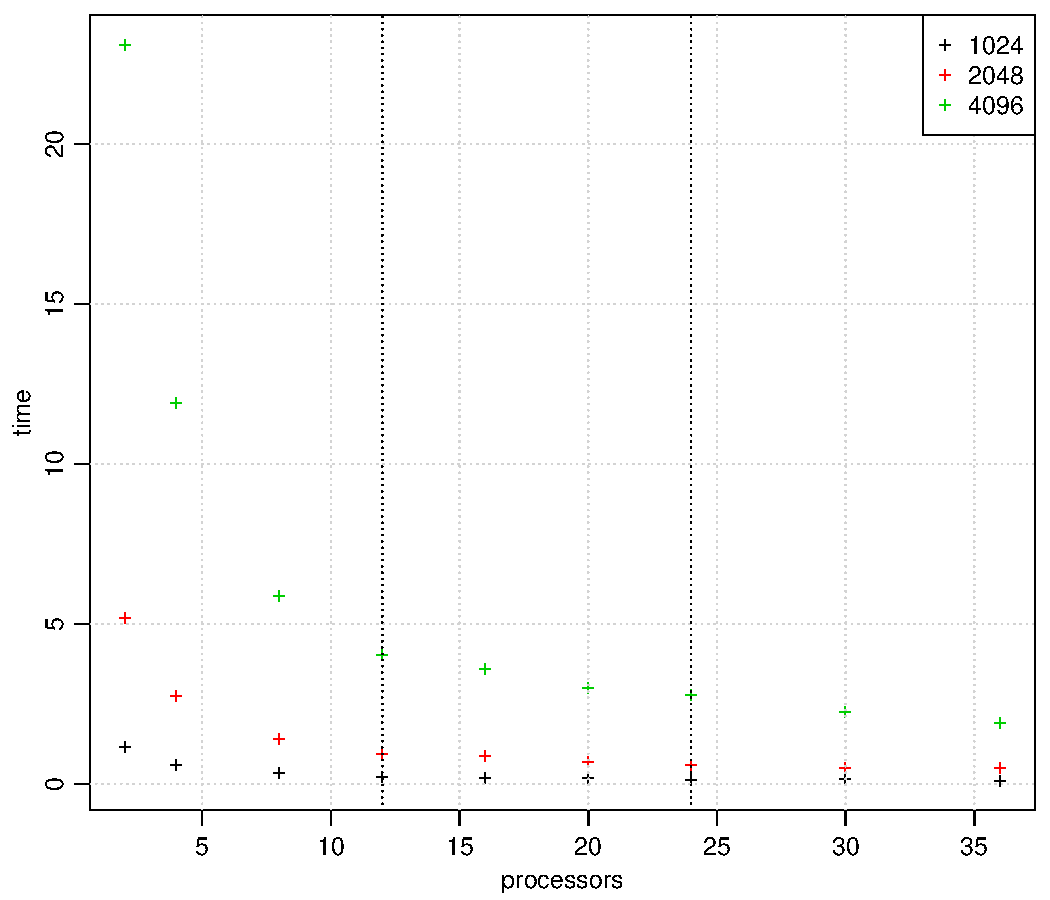
\includegraphics[width=\textwidth]{./Figures/taskbTimeProc2.pdf}
    \caption{}
    \label{fig:time2}
  \end{subfigure}
  \quad
  \begin{subfigure}[b]{0.48\textwidth}
    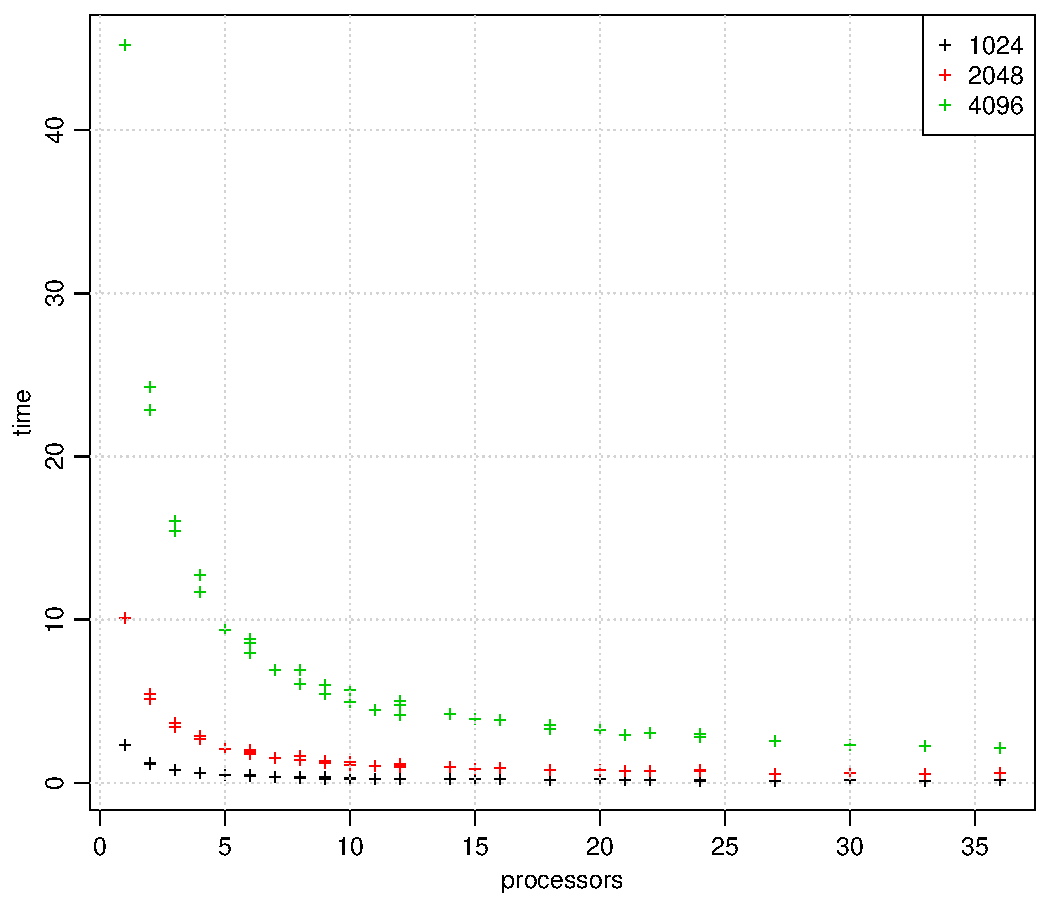
\includegraphics[width=\textwidth]{./Figures/taskbTimeNodesTimesThreads.pdf}
    \caption{}
    \label{fig:time3}
  \end{subfigure}
          %(or a blank line to force the subfigure onto a new line)
  \vspace{-0.1\baselineskip}
  \caption{Times for running problem with different amount of processes. In the upper left figure each process has one thread, while in the upper right, each process has two treads. The problem is run on as few nodes as possible, and the processes are identically distributed among the nodes. The problem size $n$ is specified in the plots. The vertical lines separate the domain to show when 1, 2 and three nodes are used. In the bottom figure only one MPI process is run per node. Between 1 and 12 threads are run on each node.}
  \label{fig:Times}
\end{figure}
\\
While Figure~\ref{fig:Times} displays the times, it is hard see much from the plots. Another diagnostics tool is to plot the \textit{speedup} $t_1/t_i$, where $t_i$ is the time used by point $i$. If there is perfect speedup, i.e. for $i$ processes the time $t_i = t_1/i$, then the speedup should be a linear function of nr. of processes, with slope 1. The speedup, along with a reference line of slope 1, is plotted in Figure~\ref{fig:Speedup}.The setup is exacly the same as in Figure~\ref{fig:time}. Here it is clear that the speedup is better for larger problem sizes. This makes sense as the overhead becomes less significant as the time increases. Also note that there are some noisy points, especially for the smallest problem size. This was addressed in the beginning of this section. What is clear here is that the noise has a higher impact on small problems as the time is shorter, which makes perfect sense. Also here it is clear that there are more overhead when problem is done on one more node (see points after vertical lines in upper left figure). However, this is not the case for the red crosses. Whether this is noise of not is hard to say.\\
%
\begin{figure}[h!]
  \centering
  \begin{subfigure}[b]{0.48\textwidth}
    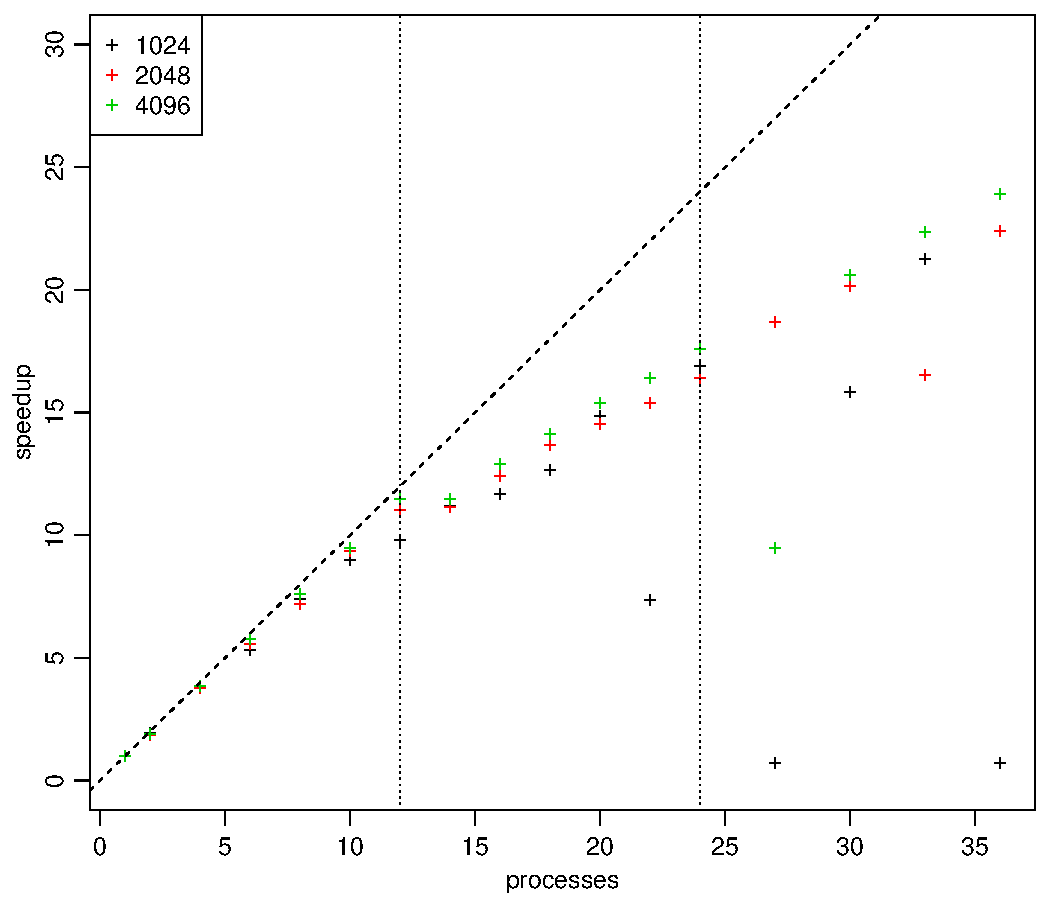
\includegraphics[width=\textwidth]{./Figures/taskbSpeedupProc1.pdf}
  \end{subfigure}%
  \quad
  \begin{subfigure}[b]{0.48\textwidth}
    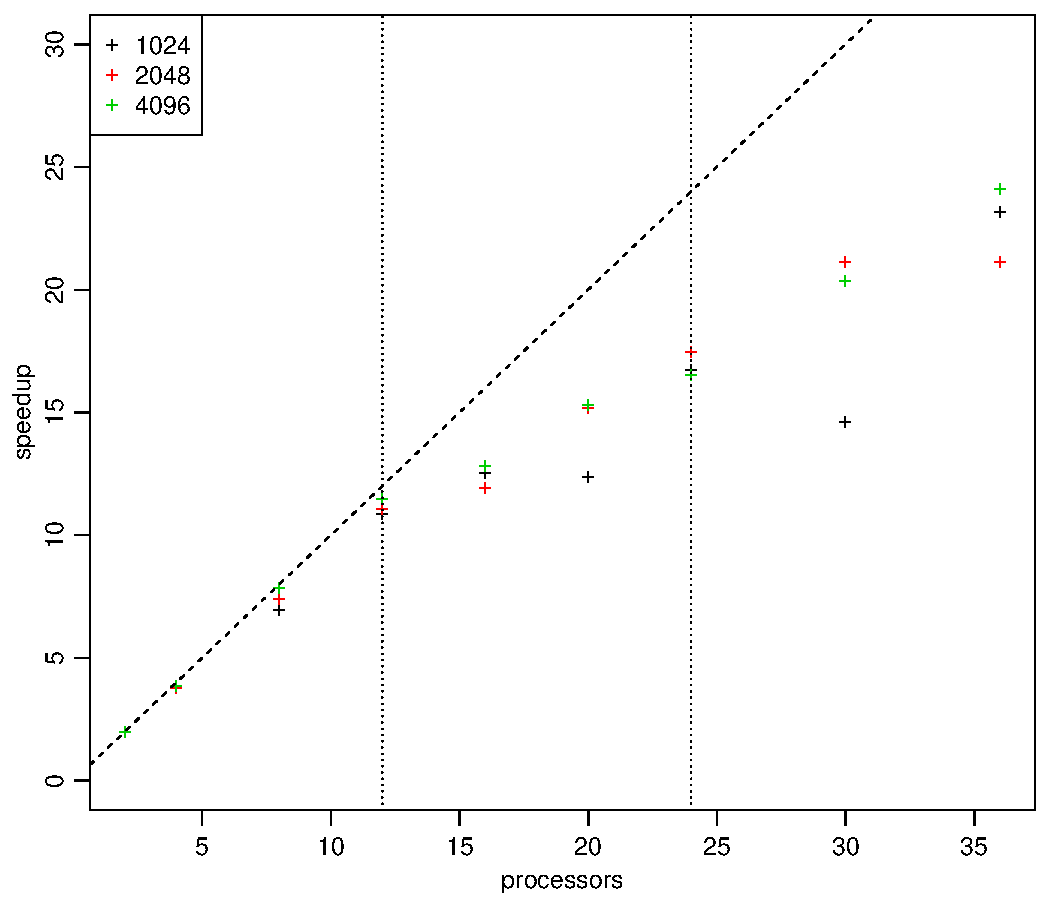
\includegraphics[width=\textwidth]{./Figures/taskbSpeedupProc2.pdf}
  \end{subfigure}
  \quad
  \begin{subfigure}[b]{0.48\textwidth}
    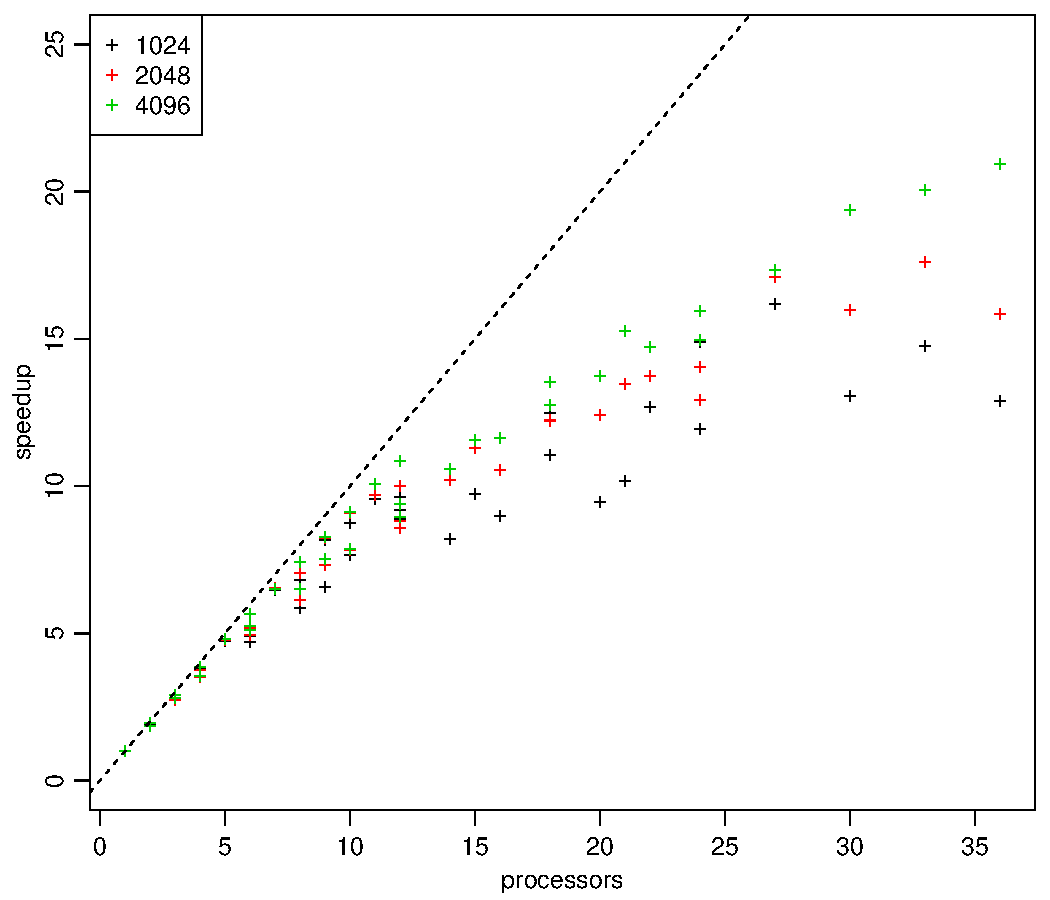
\includegraphics[width=\textwidth]{./Figures/taskbSpeedupNodesTimesThreads.pdf}
  \end{subfigure}
          %(or a blank line to force the subfigure onto a new line)
  \vspace{-0.1\baselineskip}
  \caption{Speedup for running problem with different amount of processes. In the upper left figure each process has one thread, while in the upper right, each process has two treads. The problem is run on as few nodes as possible, and the processes are identically distributed among the nodes. There are drawn vertical lines to show when a new node is utilized, and a line with slope 1. The problem size $n$ is specified in the plots. In the bottom figure only one MPI process is run per node. Between 1 and 12 threads are run on each node.}
  \label{fig:Speedup}
\end{figure}
%
\\
Another diagnostics tool is to divide the speedup by number of processes. This is called the efficiency and is 1 if the speedup is perfect. This is shown in Figure~\ref{fig:Efficiency}. The plots show pretty much the same as Figure~\ref{fig:Speedup}, but the scale is different, so it is easier to see that there is no case of perfect speedup.
\\\colorbox{yellow}{Anything else to say here? Why do we need it?}
\\
\begin{figure}[h!]
  \centering
  \begin{subfigure}[b]{0.48\textwidth}
    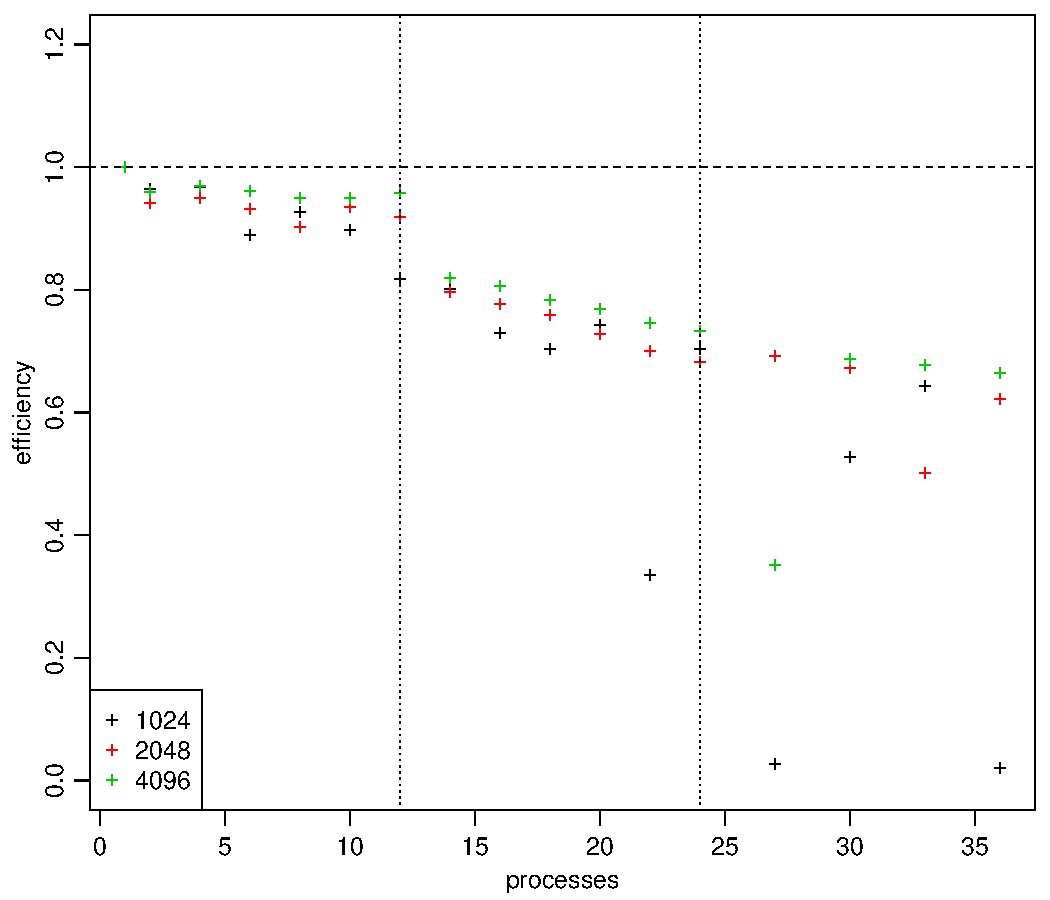
\includegraphics[width=\textwidth]{./Figures/taskbEfficiencyProc1.pdf}
  \end{subfigure}%
  \quad
  \begin{subfigure}[b]{0.48\textwidth}
    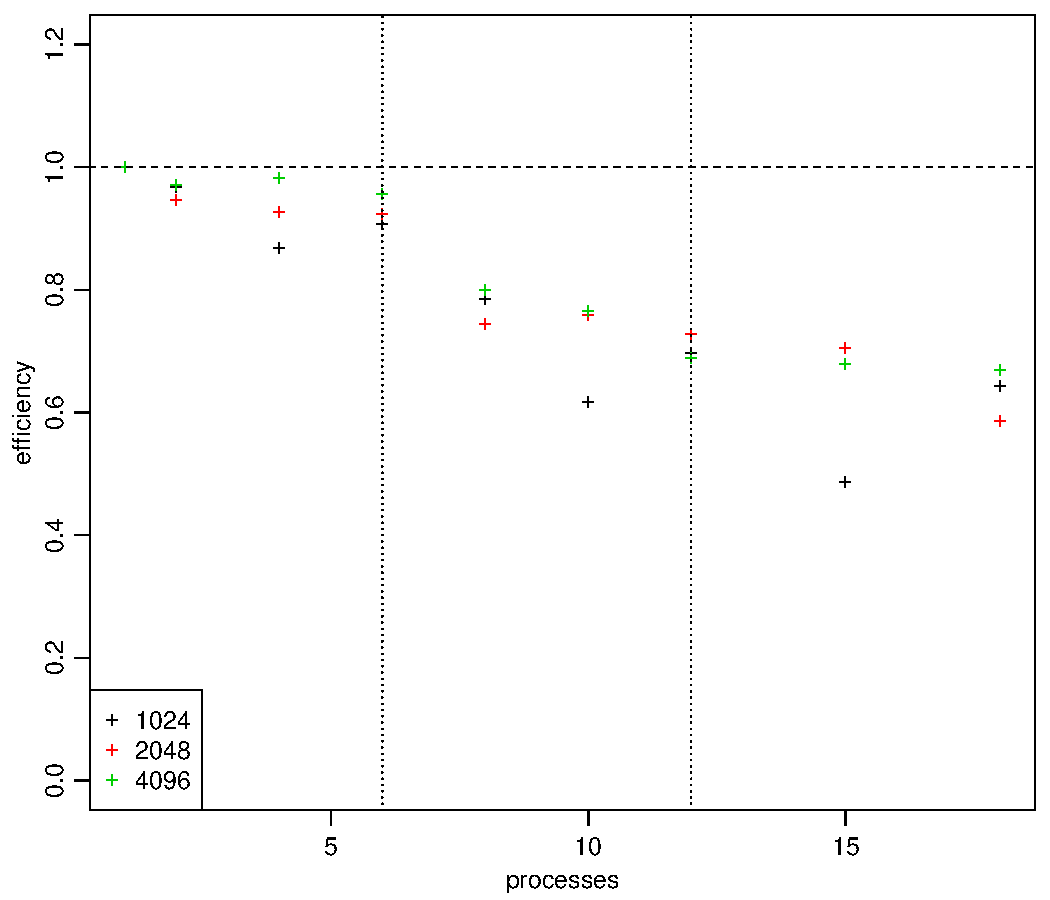
\includegraphics[width=\textwidth]{./Figures/taskbEfficiencyProc2.pdf}
  \end{subfigure}
          %(or a blank line to force the subfigure onto a new line)
  \vspace{-0.1\baselineskip}
  \caption{Efficiency for running problem with different amount of processes. In the upper left figure each process has one thread, while in the upper right, each process has two treads. The problem is run on as few nodes as possible, and the processes are identically distributed among the nodes. There are drawn vertical lines to show when a new node is utilized, and a horizontal line at 1. The problem size $n$ is specified in the plots. In the bottom figure only one MPI process is run per node. Between 1 and 12 threads are run on each node.}
  \label{fig:Efficiency}
\end{figure}
%
\\
The time of the algorithm should be of order $O(n^2 \log(n)$. To investigate how the time scales with $n$, $time/n^2$ was plotted as a function of $n$. This is displayed in the left plot in Figure~\ref{fig:timeVsn}. The data used is the same as in Figure~\ref{fig:errVsn}. One can clearly see a upward trend for larger problem sizes. Therefore $time/(n^2 \log(n)$ was also plotted in Figure~\ref{fig:timeVsn}. Here the ratio looks like it is constant. So it seems like time is of order $O(n^2 \log(n)$. For small times, the overhead becomes significant, and that is probably why the first point is so much higher for 3 and 6 processes.
\begin{figure}[h!]
  \centering
  \begin{subfigure}[b]{0.48\textwidth}
    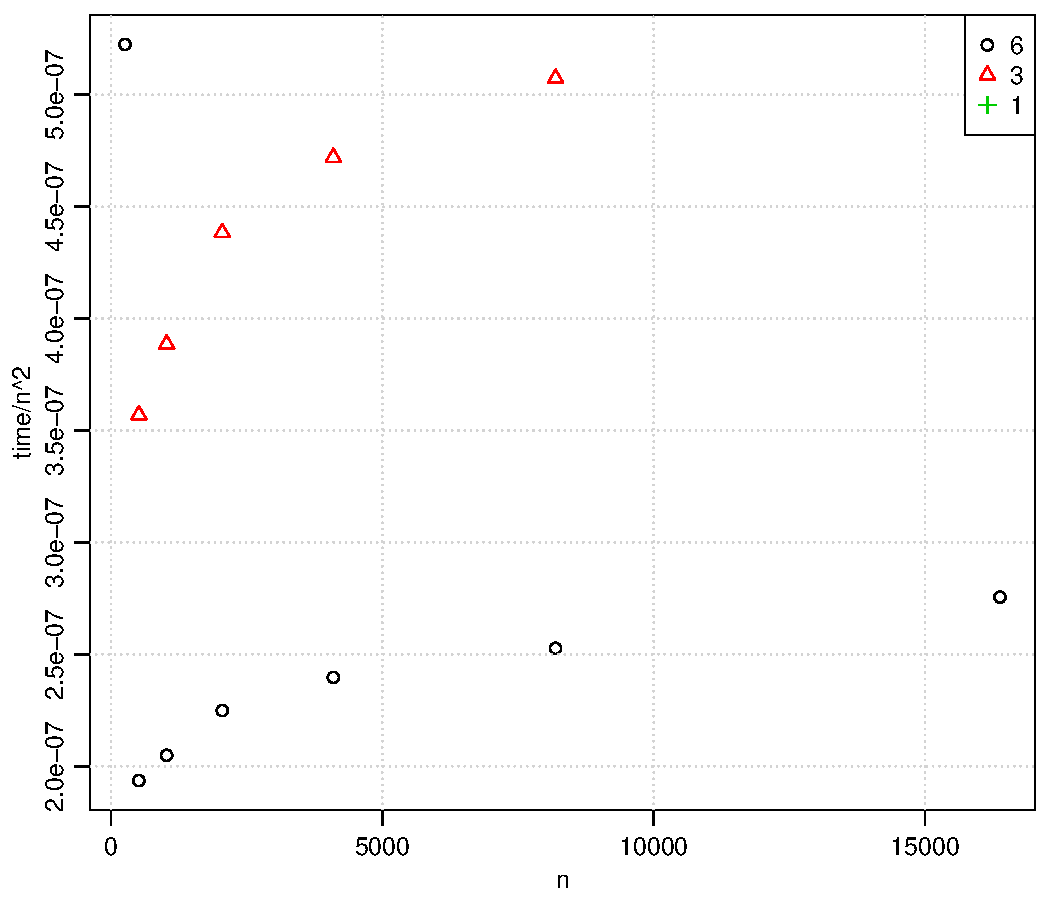
\includegraphics[width=\textwidth]{./Figures/timeOverN2Vsn.pdf}
  \end{subfigure}%
  \quad
  \begin{subfigure}[b]{0.48\textwidth}
    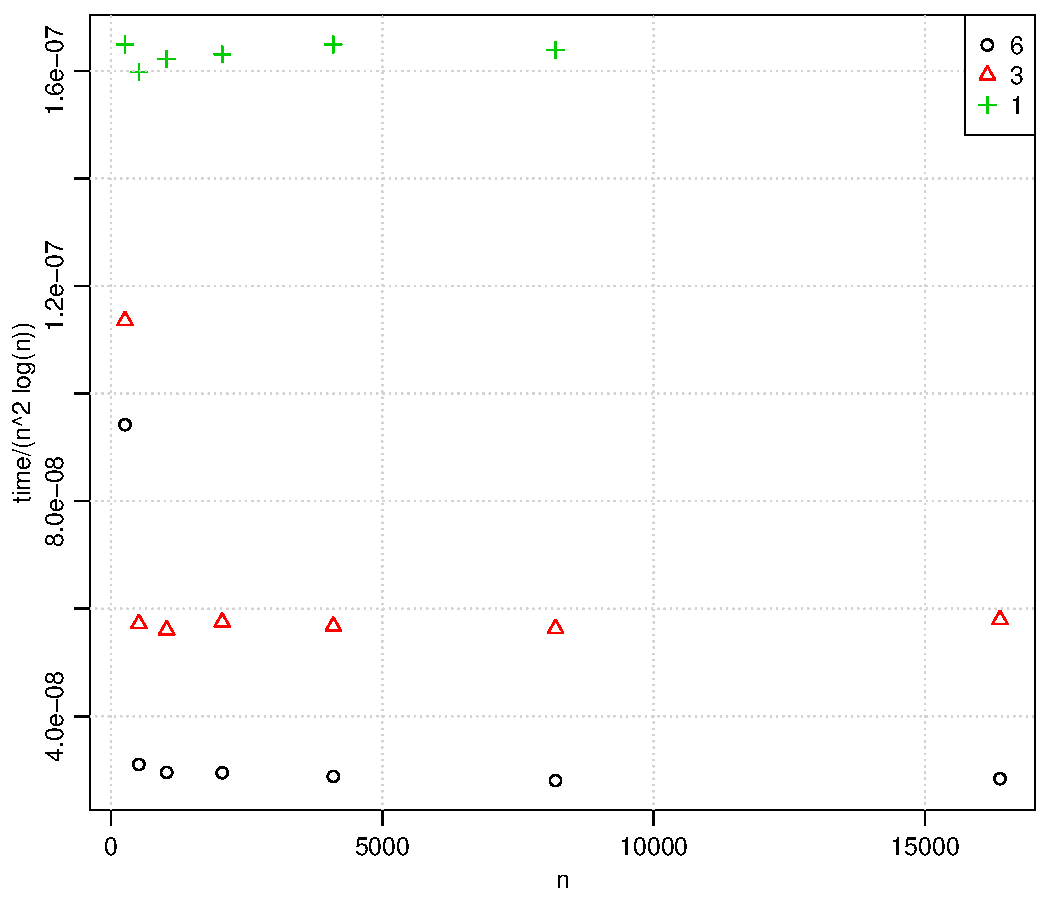
\includegraphics[width=\textwidth]{./Figures/timeOverN2LogNVsn.pdf}
  \end{subfigure}
          %(or a blank line to force the subfigure onto a new line)
  \vspace{-0.1\baselineskip}
  \caption{Left plot is $Time/n^2$ as function of $n$. Illustrates how time scales with $n^2$. The right plot is $Time/(n^2 \log (n)$. The data is the same as in Figure~\ref{fig:errVsn}.}
  \label{fig:timeVsn}
\end{figure}
